\begin{frame}{Aufgabe 2: Basisband I}
  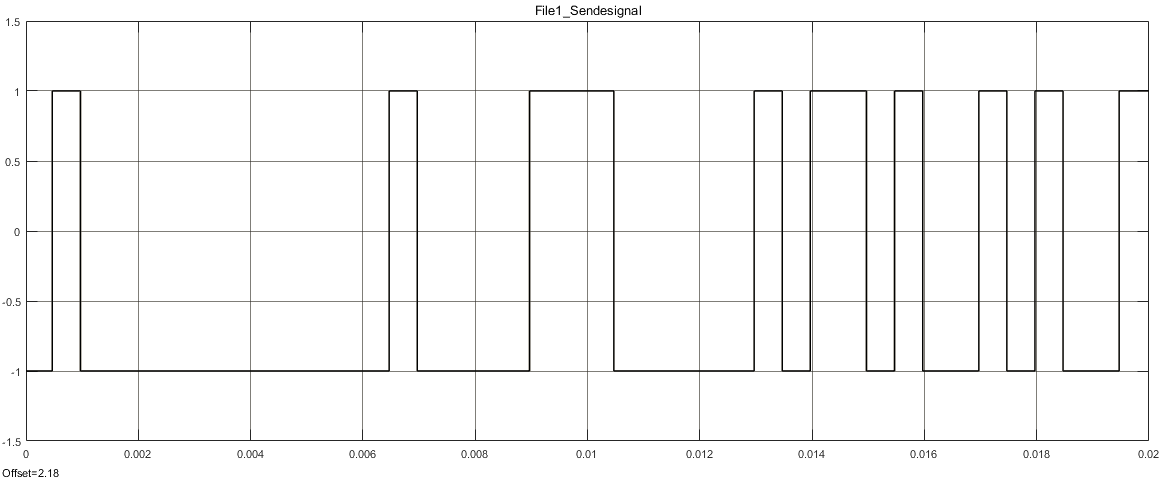
\includegraphics[width=\textwidth]{screenshots/Aufgabe2/Zeitsignal_File1}
\end{frame}

\begin{frame}{Aufgabe 2: Basisband I}
  \begin{center}
  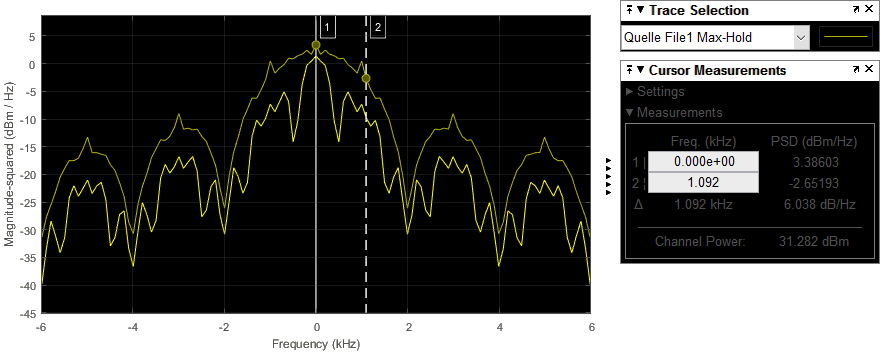
\includegraphics[height=0.4\textheight]{screenshots/Aufgabe2/Spektrum_File1}\\
  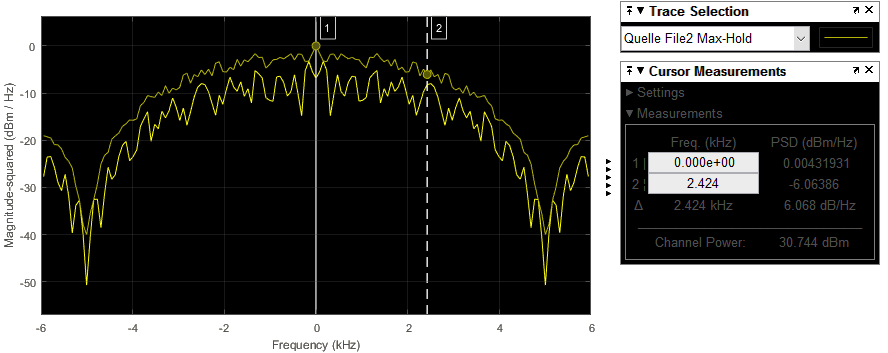
\includegraphics[height=0.4\textheight]{screenshots/Aufgabe2/Spektrum_File2}
  \end{center}
\end{frame}

\begin{frame}{Aufgabe 2: Basisband I}
  \begin{table}[H]
    \begin{tabular}{
      >{\columncolor{gray0}}l ll}
      Signal & \cellcolor{gray0}Datenrate (BR) & \cellcolor{gray0}Bandbreite ($6 \, \si{\deci\bel}$ (B)) \\
      \hline
      File 1 &  $2.001 \, \si{\kilo\bit\per\second}$                            & $1.092 \, \si{\kilo\hertz}$                              \\
      File 2    &  $5.006 \, \si{\kilo\bit\per\second}$                              &            $2.424 \, \si{\kilo\hertz}$                 
    \end{tabular}
  \end{table}

  \bigemskip
  
  Inetwa linearer Zusammenhang:\\
  \[B \approx \frac{1}{2} \cdot BR= \frac{1}{2} \cdot \frac{1}{T_S}\]
  
  \to \, Bandbreite bei $1 \, \si{\kilo\bit\per\second}$:
  \[B \approx \frac{1}{2} \cdot 1000 \, \si{\kilo\bit\per\second} = 500 \, \si{\hertz}\]
  
\end{frame}
